% .:: Laden der LaTeX4EI Formelsammlungsvorlage
\documentclass[fs, footer]{latex4ei}
\usepackage[european]{circuitikz}

\usepackage{multirow}
\usepackage{latexnew}


% Dokumentbeginn
% ======================================================================
\begin{document}


% Aufteilung in Spalten
\vspace{-4mm}
\begin{multicols*}{4}
	\fstitle{Systemtheorie}

	\emphbox{
	\textbf{Wichtiger Hinweis}
	\\ Diese Formelsammlung ist noch in der Entwicklung und nicht prüfungstauglich ! \\ Allerdings würden wir uns über Unterstützung freuen das zu ändern. Wer Lust hat kann uns über das Kontaktformular auf www.latex4ei.de erreichen.
	}
\section{Reaktive Elemente}
% ===============================================================================================

	\subsection{Die vier zentralen Größen $u,i,q,\Phi$}
	% ----------------------------------------------------------------------
	... beschreiben die Wirkungsweise von elektronischen Bauelementen.\\ \\
	\textbf{Spannung \textit{u}}: Potentialdifferenz. Hohes zu niedrigem Potential\\
	\textbf{Strom \textit{i}}: Bewegte Ladung. Bewegungsrichtung positiver Ladung\\
	\textbf{Ladung \textit{q}}: Grundeigenschaft von Materie.\\
	\textbf{Magnetischer Fluss \textit{$\Phi$}}: Grundeigenschaft von elektr. magn. Feldern\\
		\subsubsection{Allgemeine Zusammenhänge $u,i,q,\Phi$}
		Ladung und Strom beschreiben den Zustand der Materie.\\
		Spannung und magn. Fluss beschreiben den Zustand des elekt. magn. Feldes.\\
		Kondensator ist u-gesteuert (q-gesteuert), falls für ein u (q) nur ein q (u)  existiert. \\
		Induktivität ist i-gesteuert ($\phi$-gesteuert), falls für ein i ($\phi$) nur ein $\phi$ (i) existiert. \\
		\begin{tabular}{l|l}
			$i(t) = \dot q(t)$ & $[i]=A$\\
			$q(t) = q(t_0) + \int_{t_0}^t i(\tau) \mathrm d\tau$	& $[q]=As=C$ \\ \hline
			$u(t) = \dot \Phi(t)$ & $[u]=V$\\
			$\Phi = \Phi(t_0) + \int_{t_0}^t u(\tau) \mathrm d\tau$ & $[\Phi]=Vs=Wb$ \\
		\end{tabular}




		\subsubsection{Arten von Bauelementen}
		\begin{tabular}{l|l|l|l}
			Art & Symbol & Beschr. & linear\\ \hline
			Resistivität & 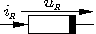
\includegraphics[height=0.4cm]{./img/Resistivitat.pdf} & $f_R(u,i)$  & $u = U_0 + R \cdot i$\\
			Kapazität & 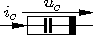
\includegraphics[height=0.4cm]{./img/Kapazivitat.pdf} & $f_C(u,q)$ & $q = Q_0 + C \cdot u$\\
			Induktivität & 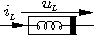
\includegraphics[height=0.4cm]{./img/Induktivitat.pdf} & $f_L(i,\Phi)$ & $\Phi = \Phi_0 + L \cdot i$\\
			Memristivität & 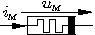
\includegraphics[height=0.4cm]{./img/Memristivitat.pdf} & $f_M(q,\Phi)$ & $\Phi = \Phi_0 + M \cdot q$\\
		\end{tabular}
		\subsubsection{Zusammenhang der Bauelemente}
		\begin{center}
			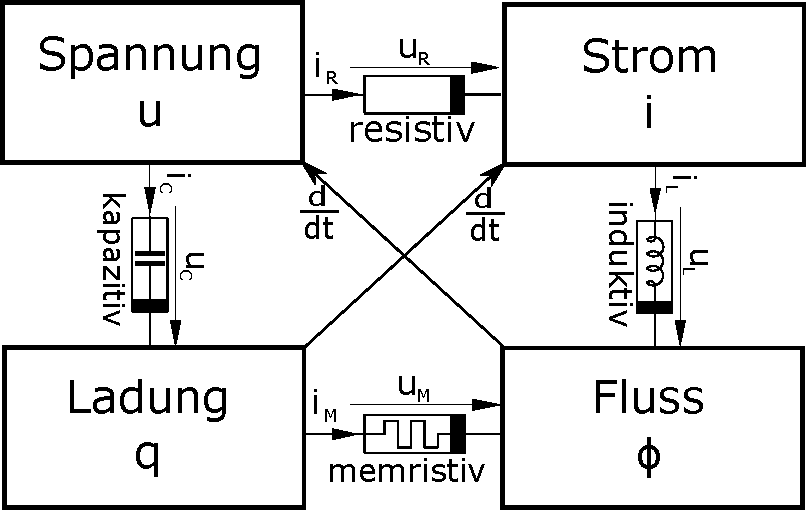
\includegraphics[scale=0.3]{./img/reactance_overview.pdf}
		\end{center}
		\subsubsection{Eigenschaften von Reaktanzen}
		\textbf{Linearität}: siehe Eintore\\
		\textbf{Differentialgleichung}: $i(t) = C \frac{\mathrm du(t)}{\mathrm dt}, u(t) = L \frac{\mathrm di(t)}{\mathrm dt}$\\
		\textbf{Gedächtnis}: Verhalten durch vorhergehende Klemmengrößen bestimmt.\\
		\textbf{Stetigkeit}: $u_C(t)$, $i_L(t)$ stetig in $(t_a, t_b)$, wenn Torgrößen endlich\\
		\textbf{Verlustfreiheit}: $W_C(t_1, t_2) = \int_{t_1}^{t_2}\! u(t)i(t)\,\mathrm dt = \int_{q_1}^{q_2}\! \mathrm{X}(q)\,\mathrm{d}t$ (Arbeit)\\
		Falls linear: $W = \frac{Cu^2}{2} = \frac{Li^2}{2}$\\
		Periodisch: $u(t+T) = u(t)$, $q(t+T) = q(t)$\\
		Graphisch: Falls keine geschlossenen Schleifen in q/u, $\Phi$/i-Diagramm existiert (Hystenesefrei)\\
		\textbf{Energie (nicht linearer Fall)}:\\
		- Kapazitiv: $W_C(t_1, t_2) = \int_{t_1}^{t_2} \! u(t)i(t)\, \mathrm dt = \int_{q_1}^{q_2} \! u(q)\, \mathrm dq$\\
		- Induktiv: $W_C(t_1, t_2) = \int_{t_1}^{t_2} \! u(t)i(t)\, \mathrm dt = \int_{\Phi_1}^{\Phi_2} \! i(\Phi)\, \mathrm d\Phi$\\
		\textbf{Energie (linearer Fall)}:\\
		- Kapazitiv: $W_C = \frac{C}{2}u^2 = \frac{1}{2C}q^2$\\
		- Induktiv: $W_L = \frac{L}{2}i^2 = \frac{1}{2L} \Phi^2$\\
		Graphisch: Fläche zwischen der Kennlinie und der q-/$\Phi$-Achse\\
		\textbf{Relaxationspunkte (=Ruhepunkte)}: Betriebspunkte, in dem die in einer Reaktanz gespeicherte Energie minimal ist. Kandidaten sind: Extremwerte, Wendepunkte, Knicke, Schnittpunkte mit q-/$\Phi$-Achse\\
		\subsubsection{Verschaltung von Reaktanzen}
		- Parallelschaltung: $C_p = C_1 + C_2$, $L_p = L_1 || L_2 = \frac{L_1L_2}{L_1+L_2}$\\
		- Serienschaltung: $C_p = C_1 || C_2 = \frac{C_1C_2}{C_1+C_2}$, $L_p = L_1 + L_2$\\


Merke: Am Kondensa\textsl{tor}, eilt der Strom \textsl{vor}, bei Induktivi\textsl{täten}, wird er sich ver\textsl{späten}\\
Merke: Ist das Mädchen brav, bleibt der Bauch konkav, hat das Mädchen Sex, wird der Bauch konvex.\\
% Liste mit Eselsbrücken für Ingenieure
% selbstausdenken begriffspaare
\section{Schaltungen ersten Grades}
\sectionbox{
	\textbf{I. Resistives ESB bestimmen}\\
\tablebox{
	\begin{tabular*}{\columnwidth}{@{\extracolsep\fill}l|ll@{}} \trule
	& Kapazität & Induktivität \\ \mrule
	ESB-Typ & Helmholtz-Thévinin & Mayer-Norton\\
	%TODO Bild einfügen :)
	Zustandsgröße & $x(t) = u_C(t)$ & $x(t) = i_L(t)$\\
	Zeitkonstante & $\tau = RC$ & $\tau = GL$\\
		\brule
	\end{tabular*}
}
	
	\textbf{II. Aufstellen DGL:} $\dot x(t) = - \fr{1}{\tau}x(t) + \fr{1}{\tau}v$ mit der Erregung $v$\\
	\textbf{III. Lösen der DGL:}\\
	Konstante Erregung:  $x(t) = x_\infty + (x_0 - x_\infty )\e^{-\frac{t-t_0}{\tau}}$ \\
	Allgemeine Erregung: $x(t) = x_0\e^{\frac{t_0-t}{\tau}}+\int_{t_0}^t{\frac{1}{\tau}v(t')\e^{\frac{t'_0-t'}{\tau}}} $ \\
	zero-input-response: Erster Summand\\
	zero-state-response: Zweiter Summand\\
	mit $u_{C,\infty}=U_0$ bzw. $i_{L,\infty}=I_0$\\
	\textbf{IV. Dynamischer Pfad}\\
\tablebox{
	\begin{tabular*}{\columnwidth}{@{\extracolsep\fill}ll@{}} \trule
	Kapazität & Induktivität\\ \mrule
	$i < 0$: $u$ wird größer & $u < 0$: $i$ wird größer\\
	$i > 0$: $u$ wird kleiner & $u > 0$: $i$ wird kleiner\\
	$i = 0$: GGP & $u = 0$: GGP\\ 	
	\brule
	\end{tabular*}
}
\textbf{Toter Punkt:} kein GGP, aber Pfad kann nicht fortgesetzt werden \ra Sprung der nicht stetigen Größe ($i_C$ oder $u_L$)\\
\textbf{Gleichgewichtspunkt (GGP):}\\
	\begin{tabular*}{\columnwidth}{@{\extracolsep\fill}ll@{}}
		Kapazität & Induktivität\\ \mrule
		$\dd{t}u_F = 0 \ra i_F = 0$ & $\dd{t}i_F = 0 \ra u_F = 0$\\
		\mrule	
	\end{tabular*}
\begin{itemize}
	\item[a)] stabil, falls der Pfad nicht aus diesem Punkt herausläuft
	\item[b)] instabil, falls der Pfad aus dem Punkt herausläuft
	\item[c)] virtuell, falls der Pfad in einen toten Punkt läuft auf dem verlängertem Pfad auf der Achse
\end{itemize}
}

\subsection{Stabile Schaltung ($\tau > 0$)}
%TODO Bilder von Graph
\subsection{Instabile Schaltung ($\tau < 0$)}
%TODO Bilder von Graph
\subsection{Dynamischer Pfad}
	
\section{Schaltungen zweiten Grades}
	\subsection{Differentialgleichungssystem aufstellen}
		\textbf{I. Schaltung umzeichnen}
		Zeichne die Schaltung so um, dass beide Reaktanzen an den äußeren Seiten sind.
		\textbf{II. Matrix aufstellen}
		(Quellen vernachlässigen)
		\begin{itemize}
		\item[a)] zwei Kondensatoren: Widerstandsmatrix $\ma R$
		\item[b)] zwei Spulen: Leitwertsmatrix $\ma G$
		\item[c)] Kondensator (Tor 1) und Spule (Tor 2): Inverse Hybridmatrix $\ma{H'}$
		\end{itemize}
		
		\textbf{III. Quellenvektor aufstellen}
		
		\textbf{IV. Differentialgleichungssystem aufstellen}
	\subsection{Phasenportraits}
		\textbf{I. Bestimmung der Eigenwerte und Eigenvektoren}\\
		\textbf{II. Bestimmung des Fixpunktes}\\
		$\ma A\v x + \ma B\v x = 0$\\
		\textbf{III. Art des Phasenportraits}\\
		%TODO Einfügen der Arten des Phasenportraits\\
		\textbf{IV. Einzeichnen von Fixpunkt und Eigenvektoren}\\
		Die Eigenvektoren werden ausgehend vom Fixpunkt eingezeichnet. Bei konjugierten Eigenvektoren zeichnet man den Realteil und den Imaginärteil.
	\subsection{Lösung der Zustandsgleichungen}
		\subsubsection{Homogener Fall}
		Transformation autonom (konst. Erregung) $\ra$ homogener Fall mit: $x' = x - x_\infty$.\\
		$\lambda_1 \neq \lambda_2$: $c_1\e^{\lambda_1t}\v q_1 + c_2\e^{\lambda_2t}\v q_2$\\
		$\lambda_1 = \lambda_2 = \lambda$: $\e^{\lambda t}(\ma 1 + (\ma A -\lambda \ma 1)t) [q_1 q_2]^T$\\
		komplexe Eigenwerte: $c_1 \e^{\alpha t}(\cos{(\beta t)}\v q_{reell} - \sin{(\beta t)}\v q_{imag} + c_2\e^{\alpha t}(\sin{(\beta t)}\v q_{reell} - \cos{(\beta t)}\v q_{imag})$\\
		%komplexe Eigenwerte: $c_1 \e^{\alpha t}( \cos{\beta t} \v{q_{reell}} - \sin{\beta t}\v q_{imaginär}) + c_2\e^{\alpha t}(\sin{\beta t}\v q_{reell} - \cos{\beta t}\v q_{imaginär})$
		\subsection{Transformation auf Normalform}
		Gegeben: $\dot{x} = \ma A\v x + \ma B\v v$\\
		Normalform: $\dot{x'} = \ma{A'}\v{x'} + \v{v'}$\\
		Eigenwerte $\lambda_1, \lambda_2$ und Eigenvektoren $\v q_1, \v q_2$ berechnen\\
		$\ma Q =  \mat{\v q_1 & \v q_2 }$\\
		$\ma{A'} = \ma Q^{-1}\ma A\ma Q = \mat{\lambda_1 & 0 \\ 0 & \lambda_2 }, \v{x'} = \ma Q^{-1}\v x$, $\v{v'} = \ma Q^{-1}\ma B\v v$.  
		\subsection{Transformation auf reellwertige Normalform}
		Gegeben: $\lambda_{1/2} = \alpha \pm \beta j, \v q_r, \v q_i$\\
		$A_{reell} =  \mat{\alpha & - \beta \\ \beta & \alpha}$\\
		$Q_{reell} = \mat{ q_r & - q_i}$\\
		$x_{reell} = \ma Q_{reell}^{-1} \e^{\Delta t}\ma Q_{reell}$\\
		$\dot{x}_{reell} (t) = A_{reell}x_{reell}(t)$\\ 
\end{multicols*}
\end{document}

